La etapa de graficación se comprende de dos pasos: el primero consiste en la captura de datos y actualización de la base de datos. El segundo paso consiste en la construcción de las gráficas en el momento en el que el usuario seleccione una de las gráficas a desplegar. Ambos pasos se llevan a cabo con apoyo de la biblioteca rrdtool de Python.

El paso de adquisición de datos y actualización de la base de datos se inicia a la par del inicio de ejecución del programa mediante la función \textbf{inicia\_captura()} mostrada en la figura \ref{image:graficar1}, perteneciente al archivo \textbf{server.py}. Esta función lee los datos de cada host del archivo \textbf{hosts.txt}, verifica por cada host si se encuentra activo y en ese caso inicia un hilo que ejecuta la función \textbf{actualizar()} del archivo \textbf{actualizarRRD.py} mostrada en la figura \ref{image:graficar2}.

\FloatBarrier
\begin{figure}[htbp!]
		\centering
			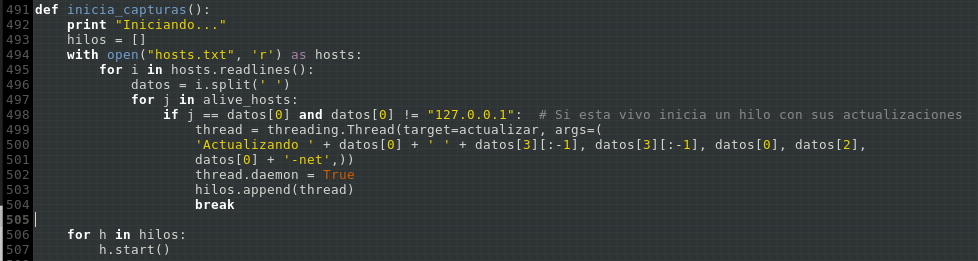
\includegraphics[width=.9 \textwidth]{images/graficar1}
		\caption{Inicio de captura de datos.}
		\label{image:graficar1}
\end{figure}
\FloatBarrier

La función \textbf{actualizar()} verifica que existe una base de datos RRD asociada al host, en caso de no existir la crea. Después, inicia por cada host activo la adquisición de datos. Estos datos son solicitados mediante la función \textbf{consultaSNMP()} del archivo \textbf{getSNMP.py} recibiendo como parámetro el OID correspondiente. Esto se muestra en la figura \ref{image:graficar4}. Las consultas SNMP se llevan a cabo cada segundo.

\FloatBarrier
\begin{figure}[htbp!]
		\centering
			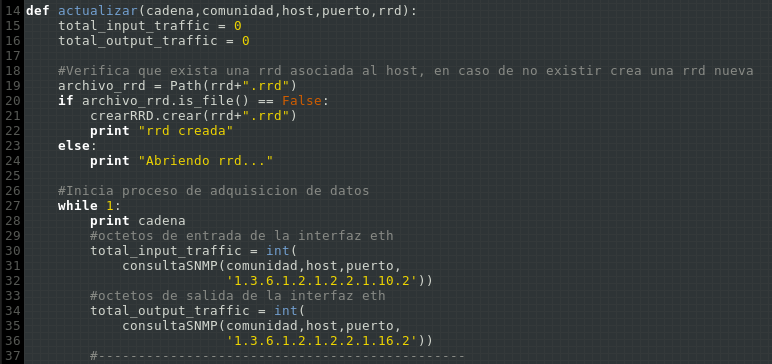
\includegraphics[width=.9 \textwidth]{images/graficar3}
		\caption{Actualización de la base de datos RRD del host.}
		\label{image:graficar2}
\end{figure}
\FloatBarrier

Una vez que se tiene el valor de la solicitud SNMP, los datos son concatenados de tal forma que la base de datos RRD los acepte. Esto se muestra en la figura \ref{image:graficar4}. Cabe mencionar que existe una base RRD por cada host activo.

\FloatBarrier
\begin{figure}[htbp!]
		\centering
			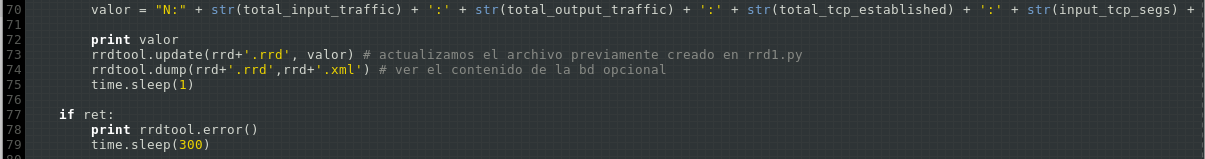
\includegraphics[width=.9 \textwidth]{images/graficar4}
		\caption{Actualización de la base de datos RRD del host.}
		\label{image:graficar3}
\end{figure}
\FloatBarrier

\FloatBarrier
\begin{figure}[htbp!]
		\centering
			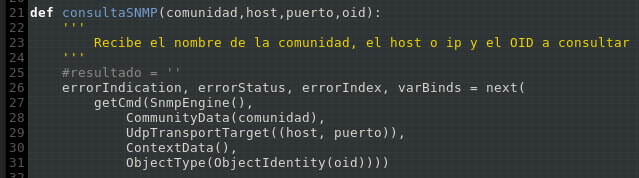
\includegraphics[width=.9 \textwidth]{images/graficar5}
		\caption{Consulta SNMP.}
		\label{image:graficar4}
\end{figure}
\FloatBarrier

Una vez que los hilos de actualización de los hosts han sido iniciados el usuario interactúa con la interfaz gráfica de la herramienta. De esta forma, al hacer clic sobre el botón \textbf{Gráficas}, el programa ejecutará la función \textbf{graphics()} del archivo \textbf{server.py}, la cual se muestra en la figura \ref{image:graficar5}.

\FloatBarrier
\begin{figure}[htbp!]
		\centering
			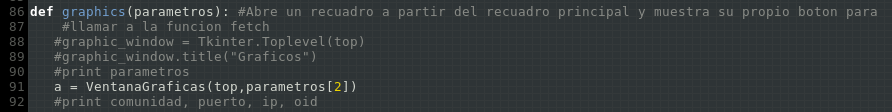
\includegraphics[width=.9 \textwidth]{images/graficar2}
		\caption{Llamada a la pantalla de selección de gráficas.}
		\label{image:graficar5}
\end{figure}
\FloatBarrier

Esta función instanciará a la clase \textbf{VentanaGraficas} del archivo \textbf{elegirGraficas.py}. Esta clase se muestra en la figura \ref{image:graficar6}. Su constructor recibe como parámetros el host (IP/Hostname) y el objeto asociado a la pantalla padre, es decir, la pantalla principal. Posteriormente, despliega los botones relacionados al tipo de gráfica a mostrar. El usuario, al seleccionar un tipo de gráfica de dicho host provocará que se ejecute el método \textbf{inicia\_ventana\_grafica()}, el cual recibe como parámetro un identificador de gráfica.

\FloatBarrier
\begin{figure}[htbp!]
		\centering
			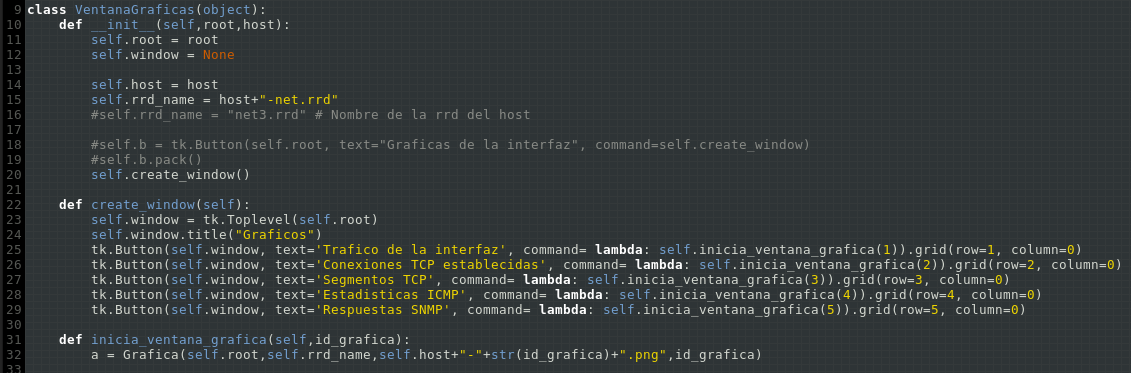
\includegraphics[width=.9 \textwidth]{images/graficar6}
		\caption{Clase para la selección de gráficas.}
		\label{image:graficar6}
\end{figure}
\FloatBarrier

El método \textbf{inicia\_ventana\_grafica()} instanciará a la clase \textbf{Grafica} del mismo archivo, como se observa en la figura \ref{image:graficar7}. La función de esta clase es iniciar un hilo en su constructor encargado de iniciar el proceso de graficación mediante el método \textbf{graficar()} del archivo \textbf{graficarRRD.py}, mostrado en la figura \ref{image:graficar8}. Una vez iniciado el proceso de graficación desplegará la ventana que refrescará cada segundo la imagen a la gráfica del host correspondiente.

\FloatBarrier
\begin{figure}[htbp!]
		\centering
			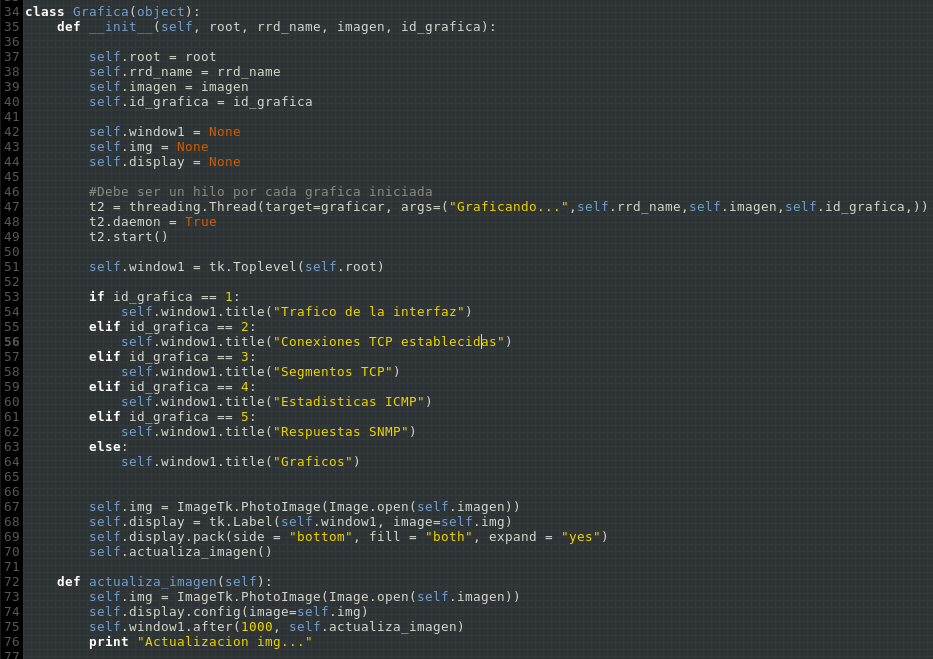
\includegraphics[width=.9 \textwidth]{images/graficar7}
		\caption{Clase para la graficación.}
		\label{image:graficar7}
\end{figure}
\FloatBarrier

Finalmente, observamos en la figura \ref{image:graficar8} que la función \textbf{graficar()} recibe como parámetro el identificador de gráfica. Esto le sirve al hilo para saber qué gráfica actualizar. La actualización se lleva a cabo con rrdtool cada segundo.

\FloatBarrier
\begin{figure}[htbp!]
		\centering
			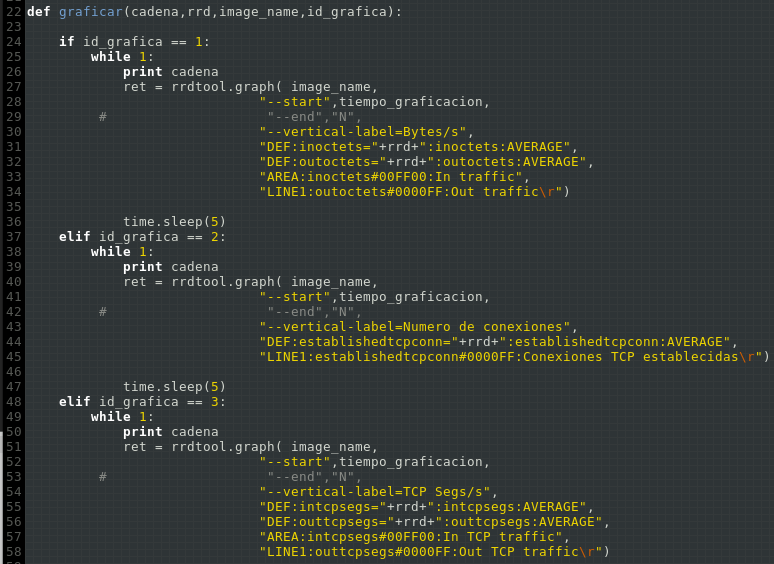
\includegraphics[width=.9 \textwidth]{images/graficar8}
		\caption{Graficación con rrdtool.}
		\label{image:graficar8}
\end{figure}
\FloatBarrier

El resultado que se muestra de los 5 objetos de la MIB elegidos por el equipo, con las gráficas en ejecución, es como el siguiente (figura \ref{image:graficas}, de igual manera, se enlistan dichos objetos:
\begin{itemize}
\item Tráfico de la interfaz
\item Conexiones TCP establecidas
\item Segmentos TCP
\item Estadísticas ICMP
\item Respuestas SNMP
\end{itemize}
\FloatBarrier
\begin{figure}[htbp!]
		\centering			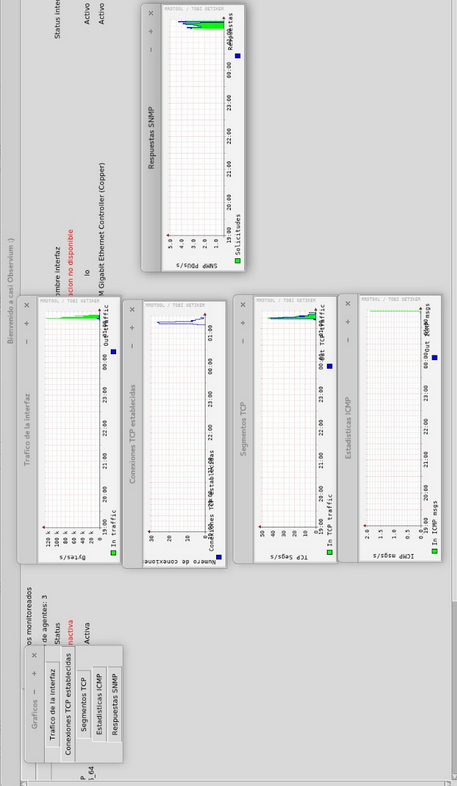
\includegraphics[width=.75 \textwidth]{images/graficas1}
		\caption{Gráficas con rrdtool.}
		\label{image:graficas}
\end{figure}
\FloatBarrier
